%\documentclass[10pt,notes]{beamer}       % print frame + notes
%\documentclass[10pt, notes=only]{beamer}   % only notes
\documentclass[11pt]{beamer}              % only frames

%%%%%% IF YOU WOULD LIKE TO CREATE LECTURE NOTES COMMENT OUT THE FOlLOWING TWO LINES
%\usepackage{pgfpages}
%\setbeameroption{show notes on second screen=bottom} % Both

\usepackage{graphicx}
\DeclareGraphicsExtensions{.pdf,.png,.jpg}
\usepackage{color}
\usetheme{winslab}
\usepackage[utf8]{inputenc}
\usepackage[english]{babel}
\usepackage{amsmath}
\usepackage{amsfonts}
\usepackage{amssymb}




\usepackage{algorithm2e,algorithmicx,algpseudocode}
\algnewcommand\Input{\item[\textbf{Input:}]}%
\algnewcommand\Output{\item[\textbf{Output:}]}%
\newcommand\tab[1][1cm]{\hspace*{#1}}

\algnewcommand{\Implement}[2]{\item[\textbf{Implements:}] #1 \textbf{Instance}: #2}%
\algnewcommand{\Use}[2]{\item[\textbf{Uses:}] #1 \textbf{Instance}: #2}%
\algnewcommand{\Trigger}[1]{\Statex{\textbf{Trigger:} (#1)}}%
\algnewcommand{\Events}[1]{\item[\textbf{Events:}] #1}%
\algnewcommand{\Need}[1]{\item[\textbf{Needs:}] #1}%
\algnewcommand{\Event}[2]{\Statex \item[\textbf{On#1:}](#2) \textbf{do}}%
\algnewcommand{\Trig}[3]{\State \textbf{Trigger}  #1.#2 (#3) }%
\def\true{\textbf{T}}
\def\false{\textbf{F}}


\author[Yağızcan Pançak]{Yağızcan Pançak\\\href{mailto:yagizcan.pancak@metu.edu.tr}{yagizcan.pancak@metu.edu.tr}}
%\author[J.\,Doe \& J.\,Doe]
%{%
%  \texorpdfstring{
%    \begin{columns}%[onlytextwidth]
%      \column{.45\linewidth}
%      \centering
%      John Doe\\
%      \href{mailto:john@example.com}{john@example.com}
%      \column{.45\linewidth}
%      \centering
%      Jane Doe\\
%      \href{mailto:jane.doe@example.com}{jane.doe@example.com}
%    \end{columns}
%  }
%  {John Doe \& Jane Doe}
%}

\title[Commit Protocols]{Commit Protocols}
\subtitle[SubTitle]{Two-Phase (2PC) and Three-Phase (3PC) Commit Protocols}
%\date{} 

\begin{document}

\begin{frame}[plain]
\titlepage
\note{In this talk, I will present .... Please answer the following questions:
\begin{enumerate}
\item Why are you giving presentation?
\item What is your desired outcome?
\item What does the audience already know  about your topic?
\item What are their interests?
\item What are key points?
\end{enumerate}
}
\end{frame}

\begin{frame}[label=toc]
    \frametitle{Outline of the Presentation}
    \tableofcontents[subsubsectionstyle=hide]
\note{ The possible outline of a talk can be as follows.
\begin{enumerate}
\item Outline 
\item Problem and background
\item Design and methods
\item Major findings
\item Conclusion and recommendations 
\end{enumerate} Please select meaningful section headings that represent the content rather than generic terms such as ``the problem''. Employ top-down structure: from general to more specific.
}
\end{frame}
%
%\part{This the First Part of the Presentation}
%\begin{frame}
%        \partpage
%\end{frame}
%
\section{Fault Tolerance in Distributed Systems}
%\begin{frame}
%        \sectionpage
%\end{frame}

\begin{frame}{Distributed Commit Problem}
\framesubtitle{The distributed commit problem refers to ensuring that all nodes in a distributed system either commit or abort a transaction together, preventing inconsistencies in data across the system.}
\begin{block}{One-Phase Commit Protocol} 
Distributed commit is often established by a coordinator. In a simple
scheme, this coordinator tells all other processes that are also involved, called
participants, whether to (locally) perform the operation in question. This
scheme is referred to as a \textbf{one-phase commit protocol}. The drawback is that if one of the participants cannot actually perform the operation,
there is no way to tell the coordinator.
\end{block}
\note{}
\end{frame}

\section{The Contribution: Two-Phase Commit Protocol (2PC)}
\begin{frame}
\frametitle{Two-Phase Commit Protocol (2PC)}
\framesubtitle{}
The Two-Phase Commit Protocol (2PC) ensures atomicity in distributed transactions efficiently. 

\begin{figure}
    \centering
    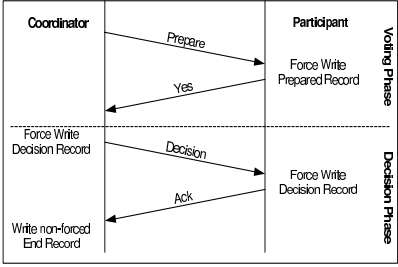
\includegraphics[scale=0.3]{figures/2PC.png}
    \caption{Two-Phase Commit Protocol (2PC)}
    \label{fig:2pc}
\end{figure}
\begin{itemize}
\item Offers a systematic approach for achieving atomicity.
\item Coordinates between a coordinator and participants.
\item Coordinator sends "prepare" message, participants respond.
\item Coordinator makes decision, sends "commit" or "abort".
\item Guarantees atomicity, minimizes inconsistencies.
\end{itemize}

\end{frame}

\section{The Contribution: Three-Phase Commit Protocol (3PC)}
\begin{frame}
\frametitle{Three-Phase Commit Protocol (3PC)}
\framesubtitle{}
The Three-Phase Commit Protocol (3PC) enhances distributed transaction atomicity with an additional phase for improved fault tolerance.

\begin{figure}
    \centering
    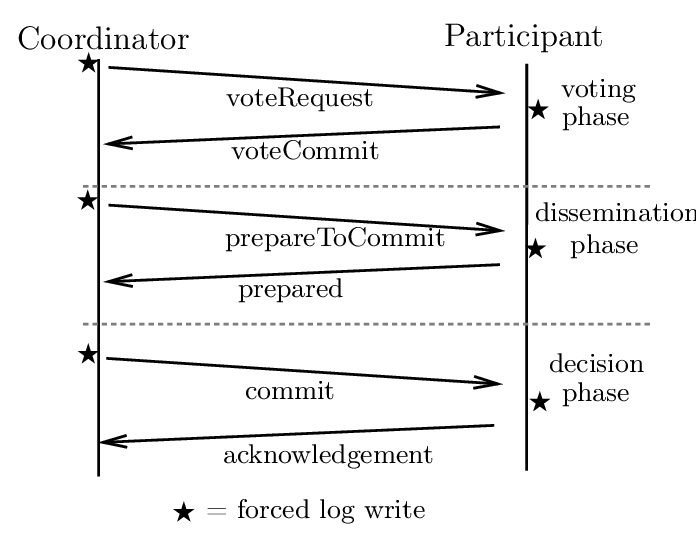
\includegraphics[scale=0.14]{figures/3PC.png}
    \caption{Three-Phase Commit Protocol (3PC)}
    \label{fig:3pc}
\end{figure}
\begin{itemize}
\item Introduces an additional phase for enhanced fault tolerance.
\item Facilitates progressive commit decisions to mitigate risks.
\item Coordinator solicits participant readiness to commit.
\item Confirms commit readiness before final decision.
\item Coordinator makes a definitive commit or abort decision.
\end{itemize}

\end{frame}


\section{Motivation/Importance}
\begin{frame}
\frametitle{Motivation/Importance}
\framesubtitle{Navigating Consensus: The Distributed Commit Challenge}
The distributed commit problem is pivotal in ensuring agreement among system nodes on transaction outcomes in distributed systems. It poses philosophical questions about autonomy versus consensus and is addressed by models like the commit protocols, despite limitations. Its applications are widespread, but its complexity stems from reconciling consensus in fault-prone distributed environments, emphasizing the need for nuanced solutions.
\end{frame}

\section{Background/Model/Definitions/Previous Works}


\subsection{Model, Definitions}

\frame{
\frametitle{Model, Definitions}
\framesubtitle{Formal definition of Commit Protocol}

\textbf{Coordinator:} Initiates and coordinates the distributed transaction by communicating with participating nodes to ensure consistency.

\textbf{Nodes:}  Participate in the distributed transaction by responding to the coordinator's messages, executing transactional operations, and maintaining transactional integrity.

\textbf{Prepare Phase:} The coordinator sends a "prepare" message to all participants, asking if they are ready to commit the transaction. Each participant replies with either a "yes" or "no" message.

\textbf{Can Commit Phase:}  The coordinator asks participants if they can commit the transaction without actually committing it. Participants reply with "yes" or "no".

\textbf{Commit Phase:} If all participants reply "yes" during the "can commit" phase, the coordinator proceeds with the commit phase; otherwise, it aborts the transaction.
}

\subsection{Background, Previous Works}
\begin{frame}{Background}

\begin{itemize}
    \item The Two-Phase Commit protocol ensures atomicity in distributed systems by employing two phases: prepare and commit, as introduced by Gray 1978 \cite{gray_1978}.

    \item The Three-Phase Commit protocol enhances the Two-Phase Commit by introducing a pre-commit phase, reducing the likelihood of blocking in case of coordinator failure, as proposed by Skeen 1981\cite{skeen_1981}
\end{itemize}

\end{frame}




\section{Contribution}

\subsection{Safety}
\begin{frame}{Safety}
\framesubtitle{Atomicity and Durability}
Both the Two-Phase Commit and Three-Phase Commit protocols ensures atomicity and durability of transactions. Atomicity means that either all nodes commit the transaction or none do, avoiding partial commits. Durability ensures that once a transaction is committed, it remains so even in the face of failures.

\end{frame}


\subsection{Fault Tolerance}

\begin{frame}
\frametitle{Fault Tolerance}
If the coordinator fails after making a decision but before notifying all cohorts, it can lead to a blocking situation known as the "blocking coordinator" problem, where some cohorts are uncertain about the status of the transaction. 

The Three-Phase Commit protocol enhances the reliability of distributed transactions by introducing a third phase, thereby addressing the blocking coordinator problem. It ensures that even if the coordinator fails after making a decision but before final commitment, the cohorts can eventually reach a consistent decision regarding the transaction's outcome.

\end{frame}




\section{Experimental results/Proofs}

\subsection{Time Complexity}
\begin{frame}
\frametitle{Time Comparison}
\begin{figure}
    \centering
    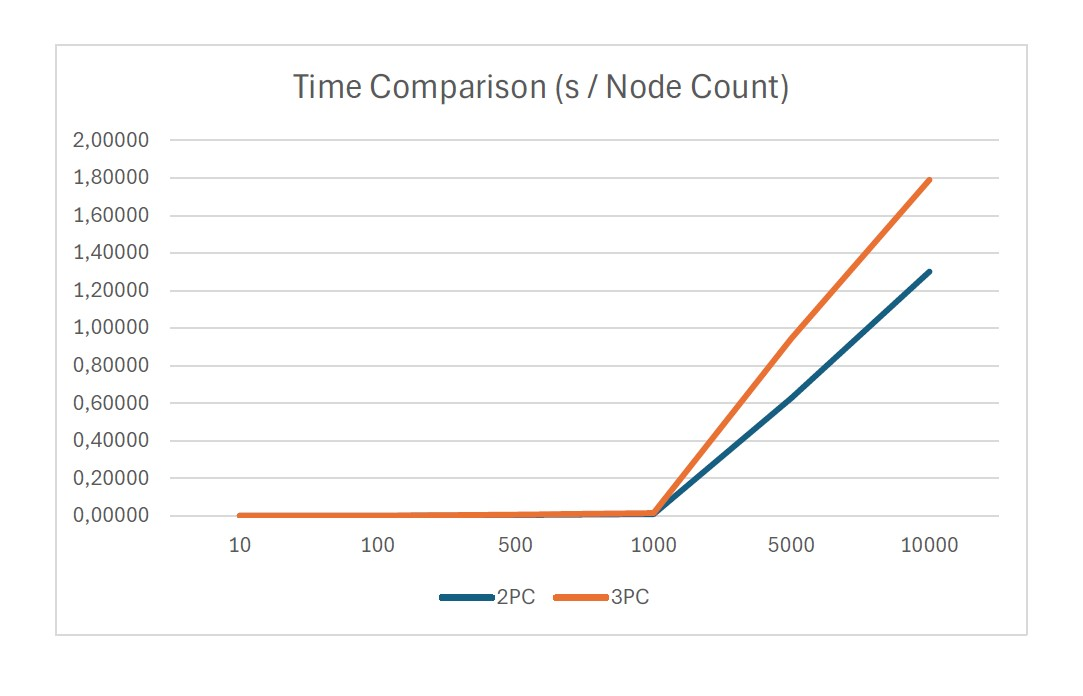
\includegraphics[scale=0.44]{figures/3PC_test.jpg}
    \caption{Simulation results for Commit Protocols}
    \label{fig:3pc_test}
\end{figure}
\end{frame}







\section{Conclusions}
\begin{frame}
\frametitle{Conclusions}
In conclusion, both the Two-Phase Commit (2PC) and Three-Phase Commit (3PC) protocols are vital for ensuring the atomicity and reliability of distributed transactions. While 2PC offers a basic framework, 3PC enhances fault tolerance by introducing an additional phase, addressing potential coordinator failures. Understanding these protocols is essential for designing robust distributed systems.

\end{frame}

\section*{References}
\begin{frame}{References}
\tiny
\bibliographystyle{IEEEtran}
\bibliography{refs}
\end{frame}




\thankslide




\end{document}